\section{Introduction to Artificial Neural Network}



\subsection{Autodiff}

\cindex{Autodiff} is neither a numerical nor symbolic differentiation. It use numerical method calculation and use symbolic rules for differentiation, so it is partly symbolic and partly numerical. See \cite{GunesBaydin2018} for more details.


One example is $f(x_1, x_2) = \log{x_1} + x_1 x_2 - \sin{x_2}$. The computation graph is:

\begin{figure}[H]
\centering	
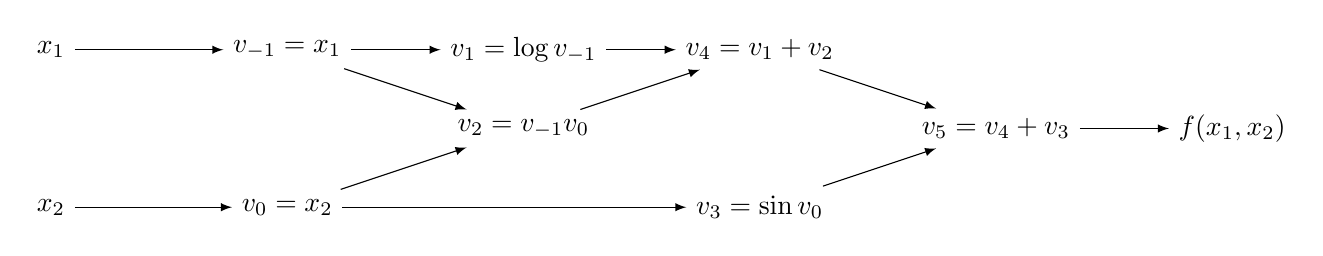
\begin{tikzpicture}
    \node (x2) at (0,0) {$x_2$};
    \node (x1) at (0,2) {$x_1$};
    \node (v0) at (3,0) {$v_0 = x_2$};
    \node (v_1) at (3,2) {$v_{-1} = x_1$};
    \node (v2) at (6,1) {$v_2 = v_{-1} v_0$};
    \node (v1) at (6,2) {$v_1 = \log{v_{-1}}$};
    \node (v3) at (9,0) {$v_3 = \sin{v_0}$};
    \node (v4) at (9,2) {$v_4 = v_1 + v_2$};
    \node (v5) at (12,1) {$v_5 = v_4 + v_3$};
    \node (final) at (15,1) {$f(x_1,x_2)$};
    \draw [-latex] (x2) -- (v0);
    \draw [-latex] (v0) -- (v3);
    \draw [-latex] (v3) -- (v5);  
    \draw [-latex] (x1) -- (v_1);
    \draw [-latex] (v_1) -- (v1);  
    \draw [-latex] (v1) -- (v4);
    \draw [-latex] (v4) -- (v5);  
    \draw [-latex] (v_1) -- (v2);
    \draw [-latex] (v2) -- (v4);
    \draw [-latex] (v0) -- (v2);
    \draw [-latex] (v5) -- (final);
\end{tikzpicture}
\caption{$f(x_1, x_2) = \log{x_1} + x_1 x_2 - \sin{x_2}$}
\end{figure}


In general there are two autodiff methods: forward mode and backpropagation. In forward mode, the derivative is the intermediary nodes against all input nodes while in backpropagation the derivative is the final node against all intermediary nodes.



\subsubsection{Forward Mode}

There are $1+n$ passes in forward mode:
\begin{enumerate}
    \item a forward evaluation of all node values. Table \ref{forwardprimaltracetable} shows the forward example.
    \item $n$ forward derivative calculation for all $n$ input features. For the $i$-th input feature, the derivatives of all $\dot{v}$ is calculated in Table \ref{forwardtangenttrace}.
\end{enumerate}

\begin{table}[H]
\centering
    \begin{tabular}{lll}
        $v_{-1}$ & $= x_1$ & $ = 2$ \\
        $v_0$ & $= x_2$ & $=5$ \\
        $v_1$ & $=\log{v_{-1}}$ & $= \log{2}$ \\
        $v_2$ & $=v_{-1} \times v_0$ & $= 2 \times 5 $\\
        $v_3$ & $=\sin{v_0}$ & $=\sin{5}$\\
        $v_4$ & $=v_1 + v_2$ & $=0.693+10$ \\
        $v_5$ & $=v_4 - v_3$ & $=10.693 + 0.959$ \\
        $y$ & $=v_5$ & $=11.652$ \\
    \end{tabular}
\caption{Forward Primal Trace}
\label{forwardprimaltracetable}
\end{table}


\begin{table}[H]
\centering
    \begin{tabular}{lll}
        $\dot{v}_{-1}$ & $= \dot{x}_1$ & $ = 1$ \\
        $\dot{v}_0$ & $= \dot{x}_2$ & $=0$ \\
        $\dot{v}_1$ & $= \displaystyle \frac{\dot{v}_{-1}}{v_{-1}}$ & $=\displaystyle \frac{1}{2}$ \\
        $\dot{v}_2$ & $=\dot{v}_{-1} \times v_0 + v_{-1} \times \dot{v}_0$ & $= 1 \times 5 + 0 \times 2$\\
        $\dot{v}_3$ & $=\dot{v}_0 \times \cos{v_0}$ & $=0 \times \cos{5}$ \\
        $\dot{v}_4$ & $=\dot{v}_1 + \dot{v}_2$ & $= 0.5 + 5$ \\
        $\dot{v}_5$ & $=\dot{v}_4 - \dot{v}_3$ & $= 5.5 - 0$ \\
        $\dot{y}$ & $=\dot{v}_5$ & $= 5.5$ \\
    \end{tabular}
\caption{Forward Tangent (Derivative) Trace}
\label{forwardtangenttrace}
\end{table}

Forward mode is expensive because it needs to run a pass for each input feature.


\subsubsection{Backpropogation}

\cindex{Backpropagation} only needs 2 passes over the calculation graph:
\begin{enumerate}
    \item a forward evaluation of all node values. The same as forward mode. Table \ref{forwardprimaltracetable} shows the forward example.
    \item a backward derivative calculation of all nodes in calculation graph. Table \ref{reverseadjointtrace} shows the backward example.
\end{enumerate}

In the backward derivative calculation, all derivatives are calculated against final result $y$. According to calculas, we have:
\begin{equation}
    \dpd{y}{v_0} = \dpd{y}{v_2} \dpd{v_2}{v_0} + \dpd{y}{v_3} \dpd{v_3}{v_0}
\end{equation}

Let $\bar{v} = \pd{y}{v}$. We have:
\begin{equation}
    \bar{v}_0 = \bar{v}_2 \dpd{v_2}{v_0} + \bar{v}_3 \dpd{v_3}{v_0}
\end{equation}

So the final result could calculated by backward propagation. Table \ref{reverseadjointtrace} gives an example.

\begin{table}[H]
\centering
    \begin{tabular}{llll}
        $\bar{v}_5$ & $=\bar{y}$ && $= 1$ \\
        $\bar{v}_4$ & $=\bar{v}_5 \pd{v_5}{v_4}$ & $=\bar{v}_5 \times 1$ & $=1$ \\
        $\bar{v}_3$ & $=\bar{v}_5 \pd{v_5}{v_3}$ & $=\bar{v}_5 \times (-1)$ & $=-1$ \\
        $\bar{v}_2$ & $=\bar{v}_4 \pd{v_4}{v_2}$ & $=\bar{v}_4 \times 1$ & $=1$ \\
        $\bar{v}_1$ & $=\bar{v}_4 \pd{v_4}{v_1}$ & $=\bar{v}_4 \times 1$ & $=1$ \\
        $\bar{v}_0$ & $=\bar{v}_3 \pd{v_3}{v_0}$ & $=\bar{v}_3 \times \cos{v_0}$ & $=-0.284$ \\
        $\bar{v}_{-1}$ & $=\bar{v}_2 \pd{v_2}{v_{-1}}$ & $=\bar{v}_2 \times v_0$ & $=5$ \\
        $\bar{v}_0$ & $=v_0 + \bar{v}_2 \pd{v_2}{v_0}$ & $=\bar{v}_0 +\bar{v}_2 \times v_{-1}$ & $=1.716$ \\
        $\bar{v}_{-1}$ & $=v_{-1} + \bar{v}_1 \pd{v_1}{v_{-1}}$ & $=\bar{v}_{-1} + \frac{\bar{v}_1}{v_{-1}}$ & $=5.5$ \\
    \end{tabular}
\caption{Reverse Adjoint (Derivative) Trace}
\label{reverseadjointtrace}
\end{table}






% Gradient Descent
\section{Gradient Descent}

\subsection{Gradient Descent Classification}

\cindex{Gradient Descent} is a numeric optimization method to calculate the minimum value of a function. For a give function $f(x)$ with gradient everywhere, if we choose $\alpha$ small enough, it is possible that $f(x') < f(x)$ where:

\begin{equation}\label{gradientdescentdefinition}
    x' = x - \alpha \nabla_x f
\end{equation}


$\alpha$ is called \cindex{learning rate}. Please be noted that the $x$ here is a vector of all input samples.


\cindex{Batch Gradient Descent} calculate the gradient of the cost function for the entire training set. So it is slow, and sometimes cannot be fit into the main memory.

\cindex{Stochastic Gradient Descent} calculate the gradient for every single training sample. So it fluctuate. 


\cindex{Mini-batch Gradient Descent} calculate the gradient for every batch of $n$ samples. It could use GPU to accelerate the training, and it is less volatile than stochastic gradient descent.

So mini-batch gradient descent is the best of all choices. However it still has the following limitations:
\begin{enumerate}
    \item The learning rate cannot be too small or too big.
    \item \cindex{learning rate schedule} is used to gradually reduce the learning rate, which mimics the \cindex{annealing}. However the training data may not match the learning schedule. 
    \item One learning rate is applied to all data. The data could be sparse or dense.
    \item Local minimum is usually not a problem. The real problem is the plateau around \cindex{saddle points}. The gradient is flat and takes long time to move away.
\end{enumerate}

So optimization algorithms is needed for an efficient gradient descent calculation.

\subsection{Gradient Descent Optimization Algorithms}

The idea of optimizing gradient descent is to change $\alpha \nabla_x f$ in Equation \eqref{gradientdescentdefinition}. We can change all of them, such as in Momentum and NAG algorithm, or change $\alpha$, such as in Adagrad, Adadelta, RMSprop, or change $\nabla_x f$, such as in Adam, AdaMax, Nadam. The popular optimization algorithms are summarized in \cite{Ruder2016}. The relationship among all these optimization algorithm is in Figure ~\ref{gradientdescentoptimizationalgorithmrelationship}.

\begin{figure}[H]
    \centering
    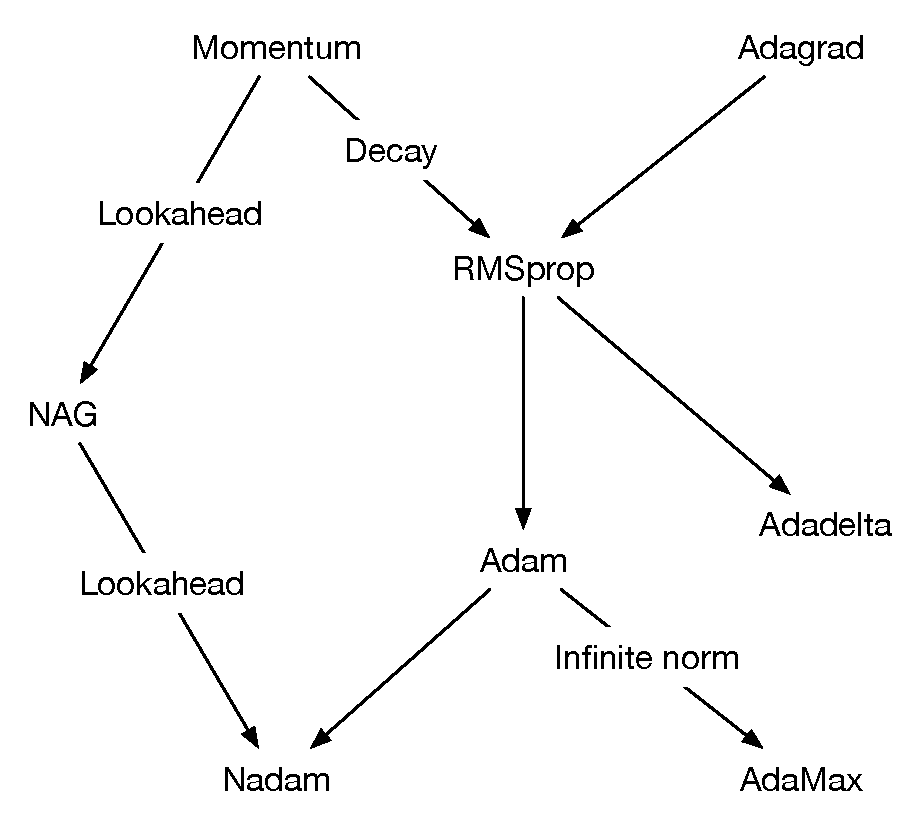
\includegraphics[scale=0.5]{images/relation_among_gradient_descent}
    \caption{Relation among Gradient Descent Algorithms}
    \label{gradientdescentoptimizationalgorithmrelationship}
\end{figure}


\subsubsection{Momentum}

\cindex{Momentum}\cite{Qian1999} takes a weighted average of all gradient:
\begin{equation}
    \begin{aligned}
        \theta_{t+1} &= \theta_t - m_t \\
        m_t &= \beta m_{t-1} + (1-\beta) \nabla_{\theta_t} J(\theta_t)
    \end{aligned}
\end{equation}

$\alpha=0.9$ for most of the cases. The momentum term increases if gradients point in the same direction and reduces updates when gradients change direction. So it has momentum when moving towards the same direction, and it converges fast.





\subsubsection{NAG}

\cindex{Nesterov Accelerated Gradient}\cite{NESTEROV1983}, or \cindex{NAG}, is a look ahead calculation. Since $\theta_t$ will be reduced by a gradient every time: $\theta_{t+2} = \theta_{t+1} - m_{t+1} = \theta_t - m_t - m_{t+1}$, it replaces $\nabla_{\theta_t} J(\theta_t)$ by $\nabla_{\theta_t} J(\theta_t - \beta m_{t-1})$:
\begin{equation}
    \begin{aligned}
        \theta_{t+1} &= \theta_t - m_t \\
        m_t &= \beta m_{t-1} + (1-\beta) \nabla_{\theta_t} J(\theta_t - \beta m_{t-1})
    \end{aligned}
\end{equation}




\subsubsection{Adagrad}

\cindex{Adagrad}\cite{Duchi2012} performs large update for infrequent and small update for frequent parameters:
\begin{equation}
    \begin{aligned}
        \theta_{t+1} &= \theta_t - \frac{\alpha}{\sqrt{G_t + \epsilon}}  \nabla_{\theta_t} J(\theta_t) \\
        G_t &= G_{t-1} + \left(\nabla_{\theta_t} J(\theta_t) \right)^2
    \end{aligned}
\end{equation}

$\epsilon$ is added to avoid division by zero. Usually $G_0 = 0$, $\alpha = 0.01$, $\epsilon = 10^{-8}$. Because $G_t$ keeps accumulating, eventually it will become too big for the algorithm to be effective.




\subsubsection{Adadelta}
\cindex{Adadelta}\cite{Zeiler2012} fixes the problem of Adagrad. It is a decay version of Adagrad:
\begin{equation}
    \begin{aligned}
        \theta_{t+1} &= \theta_t - \frac{\sqrt{D_{t-1} + \epsilon}}{\sqrt{G_t + \epsilon}}  \nabla_{\theta_t} J(\theta_t) \\
        G_t &= \beta G_{t-1} + (1-\beta) \left(\nabla_{\theta_t} J(\theta_t) \right)^2 \\
        D_t &= \beta D_{t-1} + (1-\beta) (\theta_t - \theta_{t-1})^2
    \end{aligned}
\end{equation}

Usually $G_0 = 0$, $D_0 = 0$, $\beta = 0.9$, $\epsilon = 10^{-6}$.

\subsubsection{RMSprop}

\cindex{RMSprop} is unpublished. It is a simplified version of Adadelta that $D_t = 0$:
\begin{equation}
    \begin{aligned}
        \theta_{t+1} &= \theta_t - \frac{\alpha}{\sqrt{G_t + \epsilon}}  \nabla_{\theta_t} J(\theta_t) \\
        G_t &= \beta G_{t-1} + (1-\beta) \left(\nabla_{\theta_t} J(\theta_t) \right)^2 \\
    \end{aligned}
\end{equation}

Usually $G_0 = 0$, $\alpha = 0.001$, $\beta = 0.9$, $\epsilon = 10^{-6}$.




\subsubsection{Adam}

\cindex{Adaptive Moment Estimation}\cite{Kingma2015}, or \cindex{Adam}, is yet another adaptive method:

\begin{equation}
    \begin{aligned}
        \theta_{t+1} &= \theta_t - \frac{\alpha}{\sqrt{\displaystyle \frac{G_t}{1-(\beta_2)^t}} + \epsilon} \frac{m_t}{1-(\beta_1)^t}  \\
        m_t &= \beta_1 m_{t-1} + (1-\beta_1) \nabla_{\theta_t} J(\theta_t) \\
        G_t &= \beta_2 G_{t-1} + (1-\beta_2) \left(\nabla_{\theta_t} J(\theta_t) \right)^2
    \end{aligned}
\end{equation}

Usually $G_0 = 0$, $\alpha = 0.001$, $\beta_1 = 0.9$, $\beta_2 = 0.999$, $\epsilon = 10^{-8}$.





\subsubsection{AdaMax}
\cindex{AdaMax}\cite{Kingma2015} is a infinite norm version of Adam. Adam use $l_2$ norm for $G$. For infinite norm:
\begin{equation}
    \begin{aligned}
        G_t &= \beta_2^\infty G_{t-1} + (1-\beta_2^\infty ) \norm{\nabla_{\theta_t} J(\theta_t)}^\infty  \\
        &= \max \left(\beta_2 G_{t-1}, \norm{\nabla_{\theta_t} J(\theta_t)} \right)
    \end{aligned}
\end{equation}

Because $G_t > 0$ in AdaMax, $\epsilon$ is no longer useful. So the equation could be simplified:

\begin{equation}
    \begin{aligned}
        \theta_{t+1} &= \theta_t - \frac{\alpha}{G_t}  m_t \\
        m_t &= \beta_1 m_{t-1} + (1-\beta_1) \nabla_{\theta_t} J(\theta_t) \\
        G_t &= \max \left(\beta_2 G_{t-1}, \norm{\nabla_{\theta_t} J(\theta_t)} \right)
    \end{aligned}
\end{equation}

Usually $G_0 = 0$, $\alpha = 0.001$, $\beta_1 = 0.9$, $\beta_2 = 0.999$.


\subsubsection{Nadam}

\cindex{Nadam}\cite{Dozat2016} combines Adam and NAG. Adam could be written as:
\begin{equation}
    \theta_{t+1} = \theta_t - \frac{\alpha}{\sqrt{\displaystyle \frac{G_t}{1-(\beta_2)^t}} + \epsilon} \left(\beta_1 \frac{m_{t-1}}{1-(\beta_1)^{t-1}} + \frac{1-\beta_1}{1-(\beta_1)^t} \nabla_{\theta_t} J(\theta_t) \right)
\end{equation}

Like NAG, Nadam changes Adam's $t-1$ version of $\displaystyle \frac{m_{t-1}}{1-(\beta_1)^{t-1}}$ to current $t$ version $\displaystyle \frac{m_t}{1-(\beta_1)^t}$:
\begin{equation}
    \begin{aligned}
            \theta_{t+1} &= \theta_t - \frac{\alpha}{\sqrt{\displaystyle \frac{G_t}{1-(\beta_2)^t}} + \epsilon} \left(\beta_1 \frac{m}{1-(\beta_1)^t} + \frac{1-\beta_1}{1-(\beta_1)^t} \nabla_{\theta_t} J(\theta_t) \right)  \\
        m_t &= \beta_1 m_{t-1} + (1-\beta_1) \nabla_{\theta_t} J(\theta_t) \\
        G_t &= \beta_2 G_{t-1} + (1-\beta_2) \left(\nabla_{\theta_t} J(\theta_t) \right)^2    
    \end{aligned}
\end{equation}

Usually $G_0 = 0$, $m_0 = 0$, $\alpha = 0.002$, $\beta_1 = 0.9$, $\beta_2 = 0.999$, $\epsilon = 10^{-7}$.





